\documentclass[12 pt, Times New Roman, a4paper]{article}
\usepackage[utf8]{inputenc}
\usepackage[english,russian]{babel}
\usepackage[top=2 cm, bottom = 2 cm, left = 3 cm, right = 1.5 cm]{geometry}
\usepackage{amsmath}
\usepackage{amssymb}
\usepackage{amsthm}
\usepackage[]{graphicx}
\usepackage[]{color}
\usepackage{colortbl, linegoal}
\usepackage{wrapfig}
\usepackage{listings}
\usepackage{subcaption}
\usepackage{hyperref}
\usepackage{fancyvrb}

\graphicspath{{images/}}
\renewcommand{\baselinestretch}{1.1}

\begin{document}
\subsection*{Классификация воображаемых движений}

Данные прикреплены в письме (файл alex\_long\_1.mat). Данные представляют собой записи с 24 каналами. Классифицировать данные нужно на 3 группы: воображаемое движение левой рукой, воображаемое движение правой рукой и состояние покоя.

Для запуска классификации с помощью программного обеспечения Numenta (с помощью пакета nupic для языка Python~2.7), они были преобразованы в .csv файл определенного образца. Файл также прикреплен в письме (24chan\_data\_1.csv).

Частичное описание работы с платформой Numenta и программным пакетом nupic доступно по ссылке \textbf{\href{https://github.com/numenta/nupic/wiki}{github.com/numenta/nupic/wiki}}.

Hierarchical Temporal Memory (\textbf{HTM}) --- технология, "моделирующая" работу коры головного мозга. В основе этой технолигии используется иерархическое представление отдельных "блоков памяти" (рис. \ref{fig:htm1}a). Эти блоки (или регионы) организованы как трехмерный массив (рис. \ref{fig:htm1}b). НТМ регионы также как и области коры мозга используют разреженные распределенные репрезентации, то есть в регионе активен очень малый процент "нейронов" (отдельных ячеек) одновременно.  

\begin{figure}[h]
\begin{minipage}[h]{0.49\linewidth}
\center{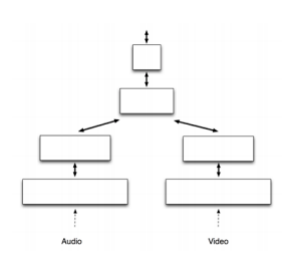
\includegraphics[width=0.5\linewidth]{hierarchy.png} \\ a) HTM}
\end{minipage}
\hfill
\begin{minipage}[h]{0.49\linewidth}
\center{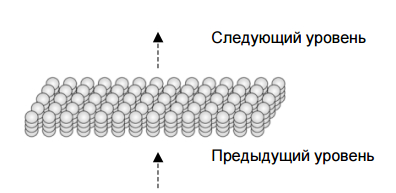
\includegraphics[width=1\linewidth]{one_region.png} \\ b) Отдельный регион}
\end{minipage}
\caption{}
\label{fig:htm1}
\end{figure}

Нижние уровни иерархии соответствуют Temporal Pooler, который отвечает за запоминание последовательностей, сильно изменяемых данных и контекстов для событий. Верхние слои соответствуют Spatial Pooler, отвечающий за обучение связей и представление более общих понятий (нежели последовательности).

Temporal Pooler используется для запоминания и предсказания на несколько шагов. В открытом коде nupic на github'е достаточно много примеров с применением пакета для предсказания некоторых данных, зависящих о времени. Для простой классификации данных используют Spatial Pooler. 

Для обозначенных в начале данных была запущена классификация. Результаты работы скрипта приведены в документе 24chan\_data\_1\_results.csv. Столбец classification отвечает за истинный класс, a столбец modelBestPrediction.0 --- за результат классификации. Я не до конца интерпретировала результат, так как в части наблюдений в полученном значении появляется не номер класса, а строка вида:\\
 \textbf{3: 0.18060211411088037\}  }
 
Но за исключением части не интерпретируемых результатов, классификация верная. Я найду путь решения проблемы, и после опишу результаты численно.

В целом, я пока подбирала параметры больше интуитивно. Далее подберу модель лучше. 
\end{document}